\documentclass[conference]{IEEEtran}
\IEEEoverridecommandlockouts
% The preceding line is only needed to identify funding in the first footnote. If that is unneeded, please comment it out.
\usepackage{cite}
\usepackage{amsmath,amssymb,amsfonts}
\usepackage{algorithmic}
\usepackage{graphicx}
\usepackage{textcomp}
\usepackage{xcolor}
\def\BibTeX{{\rm B\kern-.05em{\sc i\kern-.025em b}\kern-.08em
    T\kern-.1667em\lower.7ex\hbox{E}\kern-.125emX}}
\begin{document}

\title{Towards Better Biocommunication: Refining Electrode Technology for BioImpedance and Body-Coupled Communication\\

\thanks{Sustronics something-something}
}

\author{\IEEEauthorblockN{1\textsuperscript{st} Juris Ormanis}
\IEEEauthorblockA{\textit{Cyber-Physical Systems Laboratory} \\
\textit{Institute of Electronics and Computer Science}\\
Riga, Latvia \\
email address or ORCID}
\and
\IEEEauthorblockN{2\textsuperscript{nd} Anastasija Shevchenko}
\IEEEauthorblockA{\textit{Cyber-Physical Systems Laboratory} \\
\textit{Institute of Electronics and Computer Science}\\
Riga, Latvia \\
email address or ORCID}
\and
\IEEEauthorblockN{3\textsuperscript{rd} Krisjanis Nesenbergs}
\IEEEauthorblockA{\textit{Cyber-Physical Systems Laboratory} \\
\textit{Institute of Electronics and Computer Science}\\
Riga, Latvia \\
email address or ORCID}
\and
\IEEEauthorblockN{4\textsuperscript{th} Armands Ancans}
\IEEEauthorblockA{\textit{dept. name of organization (of Aff.)} \\
\textit{Institute of Electronics and Computer Science}\\
Riga, Latvia \\
email address or ORCID}
\and
\IEEEauthorblockN{5\textsuperscript{th} Modris Greitans}
\IEEEauthorblockA{\textit{dept. name of organization (of Aff.)} \\
\textit{Institute of Electronics and Computer Science}\\
Riga, Latvia \\
email address or ORCID}
}

\maketitle


\section{Introduction}
\input{sections/001_context.tex}
\input{sections/002_objectives.tex}
% ... more subsections as needed

\section{Materials and Methods}

To develop the benchmark for electrodes in BioZ and BCC application, first of all we need to identify what are the parameters we are seeking. In other words, if we have ideal signal, what are parameters of that signal, and what changes of those parameters would lead to reduction of quality of the signal.

Starting our thought experiment with pure sine wave, with zero noise, and amplitude high enought, so the smallest changes in that sine-wave would be captured by our ideal ADC.

Now lets observe real life measurements (See figures \ref{fig:agagcl_breathing}, \ref{fig:edigold_breathing}, \ref{fig:movsense_breathing}) and try to identify what are those elements that separates real world form ideal. 

\begin{figure}
    \centering
    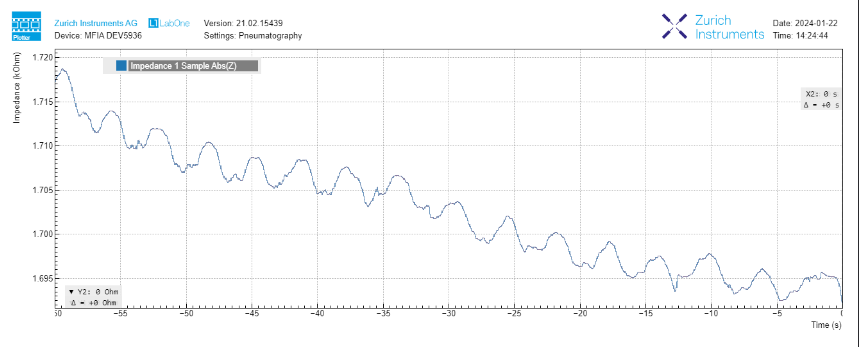
\includegraphics[width=1.2\linewidth]{figures/PlaceHolders/AgAgCl_Placeholder.png}
    \caption{AgAgCl electrodes capturing breathing}
    \label{fig:agagcl_breathing}
\end{figure}

\begin{figure}
    \centering
    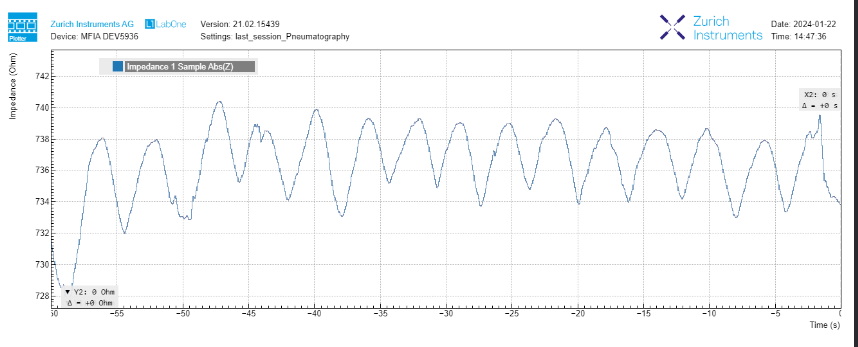
\includegraphics[width=1.2\linewidth]{figures/PlaceHolders/EDI_Gold_Placeholder.png}
    \caption{Custom, gold plated electrodes capturing breathing}
    \label{fig:edigold_breathing}
\end{figure}

\begin{figure}
    \centering
    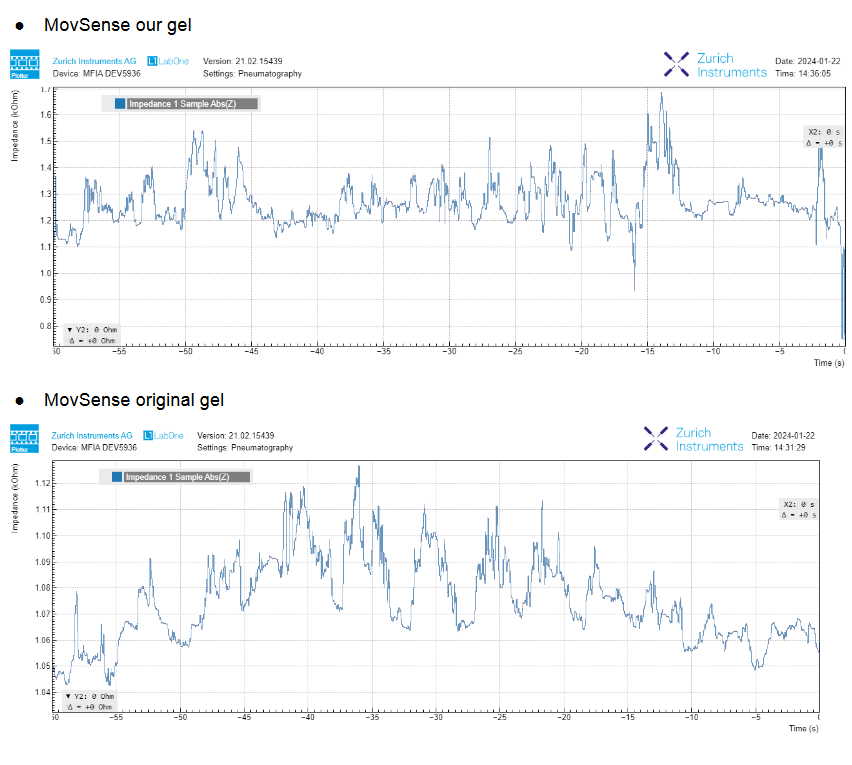
\includegraphics[width=1.2\linewidth]{figures/PlaceHolders/MovSense_Placeholder.png}
    \caption{Unknown electrodes from our shelf, we completely have no idea who is the manufacturer of those electrodes}
    \label{fig:movsense_breathing}
\end{figure}

Looking at \ref{fig:agagcl_breathing}, we see that "amplitude of inhale-exhale" is about 5 ohms, the measurement drifts from 1.72KOhm to 1.695KOhms over one minute. There is insignificant noise, about 0.1 Ohm and breathing pattern is clearly visible.

Looking at \ref{fig:edigold_breathing}, we see that "amplitude of inhale-exhale" is about 5 ohms, the measurement drifts from 734Ohm to 736Ohms over one minute. There is insignificant noise, about 0.1 Ohm and breathing pattern is clearly visible.

Looking at \ref{fig:movsense_breathing}, we are unable to see "amplitude of inhale-exhale", the measurement have no significant drift. There is drastic noise and artifacts, breathing pattern is not visible.

From those observations we can conclude that we are looking for electrodes that provides stable, low-noise, high amplitude signal.

So, to evaluate the electrodes, we will need to move from qualitative to quantitative analysis. firs of all we need to define the parameters that we are going to measure.

our proposal is to measure:
\begin{itemize}
    \item Amplitude of inhale-exhale
    \item Drift of the measurement
    \item Noise
    \item SNR
    \item Artifacts
    \item Breathing pattern visibility
    \item Heartbeat pattern visibility
    \item Muscle activity pattern visibility
    \item Skin impedance (atkartojamība)
\end{itemize}



\input{sections/011_participants.tex}
\input{sections/012_equipment.tex}
% ... more subsections as needed

\section{Experimental Design}

This section outlines the experimental procedures utilized to evaluate the performance of three distinct types of electrodes under various test conditions. The aim was to assess the electrodes' impedance characteristics and their suitability for BioImpedance (BioZ) and Body Coupled Communication (BCC) applications. Experiments were systematically conducted across six different scenarios, employing both four-terminal and two-terminal connection methods.

\subsection{Experimental Conditions}
The electrodes were evaluated under the following test conditions:
\begin{enumerate}
    \item Open Circuit - The electrodes were not connected to any medium or each other, serving as a control setup to measure the open-circuit impedance.
    \item Copper Foil - Electrodes were placed on a conductive copper foil to simulate a uniform conductive environment.
    \item Short Circuit/Flop - The electrodes were directly connected to each other, providing a zero impedance reference.
    \item Fake Skin (Phantom) - The electrodes were placed on a synthetic skin substitute that had been moistened, mimicking the electrical properties of human skin.
    \item Gel Bath - A bath of ultrasound gel served as another phantom medium, representing a different set of electrical properties for comparison.
    \item Calf Placement - Electrodes were applied to the calf of human participants. This phase of the experiment is planned for future execution.
\end{enumerate}

\subsection{Connection Methods}
Each of the above conditions was tested using the following electrode connection configurations:
\begin{enumerate}
    \item Four-Terminal Parallel - The potential (voltage) terminals were attached to one electrode, while the current terminals were attached to a separate electrode. This setup aimed to minimize the impact of electrode impedance on the potential measurement.
    \item Four-Terminal Series - The potential and current terminals on one side (Lpot and Lcur) were connected to the first electrode, whereas the potential and current terminals on the other side (Hpot and Hcur) were connected to the second electrode. This method allows for the evaluation of the combined impedance of the electrode-skin interface and the electrode itself.
    \item Two-Terminal Bipolar - A straightforward bipolar measurement was conducted by using only two terminals, which combined the current and potential measurement through the same electrodes. This configuration is commonly used in simpler impedance measurement devices but is susceptible to electrode polarization effects.
\end{enumerate}

\subsection{Procedure}
The experimental procedure for each test condition and connection method was as follows:
\begin{itemize}
    \item Setup the impedance analyzer with the appropriate connection method.
    \item Calibrate the analyzer using the open and short circuit conditions.
    \item Apply the electrodes to the medium as specified by the test condition.
    \item Perform impedance measurements across a defined frequency range.
    \item Record the impedance values and any observed anomalies.
    \item Ensure environmental conditions such as temperature and humidity are consistent throughout the experiments.
\end{itemize}

\subsection{Data Analysis}
Data collected from the impedance measurements will be analyzed to determine the performance characteristics of each electrode type. The analysis will include:
\begin{itemize}
    \item A comparison of impedance values under different test conditions.
    \item Assessment of the repeatability and reliability of the measurements.
    \item Statistical analysis to evaluate the significance of the observed differences.
\end{itemize}

\subsection{Future Work}
The upcoming calf placement experiments will involve:
\begin{itemize}
    \item Applying electrodes to the calves of human participants after obtaining ethical approval and informed consent.
    \item Repeating the impedance measurements and comparing them with the phantom models.
    \item Analyzing the in vivo data in the context of the previous phantom experiments.
\end{itemize}

The results from these comprehensive experiments will inform the development of optimized electrodes for BioZ and BCC applications.

\end{document}

\section{Results}
% Results content goes here, or include subsections

\section{Discussion}
% Discussion content goes here, or include subsections

\section{Conclusion}
% Conclusion content goes here


\bibliographystyle{IEEEtran}
\bibliography{IEEEabrv,IEEEexample}

\end{document}